\section{Results and discussion} \label{sec:measure}
In the previous section, we detailed our implementation based on the pruning scheme and the algorithm developed in Section \ref{sec:design}. In this section, we determine if the design objectives are met by measuring the outputs and performance of the proposed accelerator.

First, we describe the experimental setup to measure the performances of the proposed architecture. Second, we show the obtained results and what observations can be made. Finally, a discussion of the obtained results is done.
%
\subsection{Experimental setup} \label{subs:exp_set}
%
After having developed the architecture on SystemVerilog, we can perform a functional simulation using a testbench (see Section \ref{sec:fpga}). This functional simulation allows us to first verify if the output of the design is logically correct (fourth design objective) and if the pruning increases the performance of the inference by measuring the number of cycles required to execute the layer (fifth design objective). Indeed, if we increase the sparsity, we should expect a reduction in the number of cycles to execute the inference.

This functional simulation was done using \textsc{ModelSim-Altera}, an \acrshort{hdl} simulation environment. The software simulates the testbench and proposed accelerator as implemented on an \acrshort{fpga}. Using this simulation, we can extract the required results.

Before checking if the design objectives are met, we must choose the target platform on which the design is implemented. According to \textcite{liu_fpga-based_2019}, the most commonly used architecture for \acrshort{dl} is a heterogeneous system. It combines both a \acrshort{cpu} and an accelerator (\acrshort{fpga}). Therefore, we chose DE10-Nano for this reason. This platform integrates a \acrfull{hps} (Dual-core ARM* Cortex*-A9 MPCore), an \acrshort{fpga} (Cyclone V 5CSEBA6U23I7N), and a 1GB DDR3 memory \cite{technologies_terasic_nodate}. The external memory is large enough to store the \acrshort{cnn} data, according to the conclusions made in Section \ref{subs:extmem}. However, in the frame of the thesis, we focus only on the accelerator part.

Since we perform a functional simulation of the accelerator part of the design, we have to also simulate the behavior of the external memory (DDR3) using the testbench. This was done by first creating files using a Python script which contains the weights and input data of the bottleneck convolution (one file for each type of data). A Python script was written to produce random input \acrshort{fm} and weight filters. Therefore when the simulation is performed, if the \acrshort{dma} requests data at a particular address, the testbench reads the data at this address in the corresponding file. Since each data type is specified by its offset (see Section \ref{subs:extmem}), we can easily determine based on the address which files to read.

In the same manner, when the \acrshort{dma} writes the output \acrshort{fm} tile into the external memory, the testbench writes the tile into a file with the corresponding address to reconstruct the output \acrshort{fm}. To verify if the output \acrshort{fm} is logically correct, a Python script was developed to compute the correct output. Therefore, we can compare both results and determine the correctness of the accelerator.

As said in Section \ref{subs:quantization}, all pixels and weights are represented using $16$ bits. Since the DDR3 memory stores words of $32 \ bits$, it is sufficient to store each type of data in using a single address.

Table \ref{tab:param} lists the parameters chosen to produce the results. Since the goal is to assess the correctness of the output of the network and measure its performance, we can choose arbitrary dimensions for input and output \acrshort{fm}s. I chose parameters that are not too small to be able to observe distinct results and not too large for the sake of the latency of the functional simulation. However, the design made is parametrizable and those parameters can be easily modified.
%
\begin{table}[H]
    \centering
    \begin{tabular}{|c|c|}
    \hline
    $N_{ix}, N_{iy}$ & 7 \\
    \hline
    $N_{if} $ & 32 \\
    \hline
    $N_{of}$ & 64 \\
    \hline
    $S$ & 1\\
    \hline
    $t$ & 6 \\
    \hline
    $T_{ox}, T_{oy}$ & 16 \\
    \hline
    \end{tabular}
    \caption{Parameters of the implemented layer}
    \label{tab:param}
\end{table}
%
\subsection{Results} \label{subs:res}
In this section are presented the results obtained from the functional simulation of the design using parameters from Table \ref{tab:param}. First, we present the comparison between expected and obtained output \acrshort{fm}, to check if the proposed architecture provides a logically correct output (fourth design objective). Second, we compare the performance of the network by modifying the pruning parameters to observe if an increase in the sparsity improves the performance of the architecture (fifth objective). Finally, we look at the resource usage of the network to see if the design can be implemented on the target platform.
%
\subsubsection{Logical correctness of the design}
%
As explained previously, the logical correctness is measured by comparing the expected output \acrshort{fm} of the network (generated by a Python script that performs the proposed bottleneck convolution using floating-point numbers) with the obtained output \acrshort{fm} (generated by the functional simulation of the network using the same input \acrshort{fm} and filters as the Python script). Since fixed-point arithmetic is more subject to arithmetic error than floating-point numbers, the obtained output pixels can be less precise than the expected ones. We consider therefore that an obtained output pixel is correct if the difference between the obtained and expected output pixel is below a threshold, which was at $0.1$.

We illustrate the ratio of correct output pixel depending on the number of partial sums per output pixel in Figure \ref{fig:res-output}, where the number of partial sums per output pixel represents the number of partial products we need to add to the partial result of the depthwise convolution to obtain a final output pixel. In other words, it is equal to $N_{np} \times N_{gr-int}$.
%
\begin{figure}[H]
    \centering
    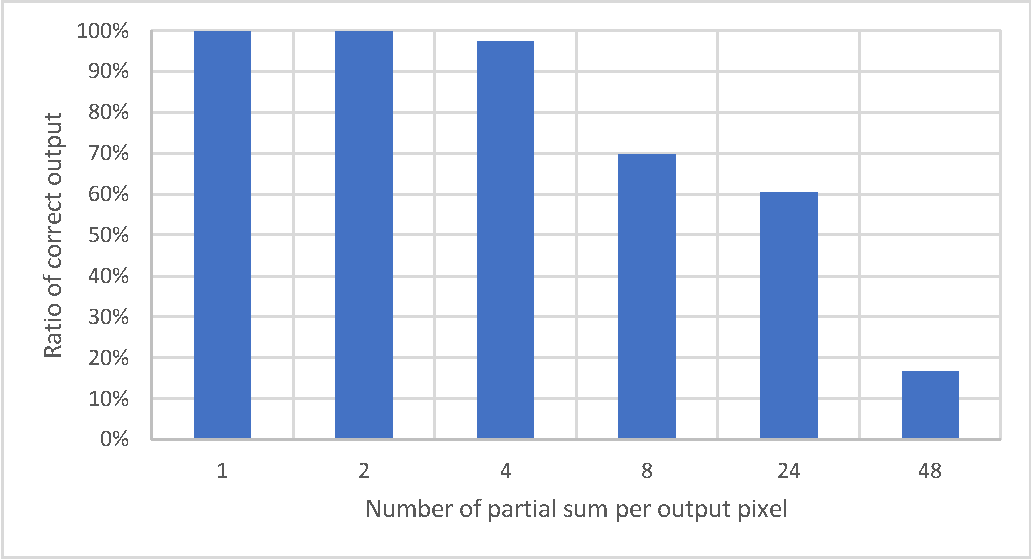
\includegraphics[width=0.8\textwidth]{ratio_correct_output.pdf}
    \caption{Ratio of correct output depending on the number of partial sums per output pixel}
    \label{fig:res-output}
\end{figure}

We can observe in Figure \ref{fig:res-output} that the ratio of correct output is almost maximal for small numbers of partial sum, but as this number increases the ratio of correct output drops rapidly. It can be explained by the accumulation of small rounding errors which leads to a drop in precision. This is verified by the fact that a bigger threshold increases the ratio of correct output. For example, if the threshold = $2$, the ratio of correct output becomes equal to $80\%$ when the number of partial sums is equal to $48$. In Figure \ref{fig:res-output}, where threshold = $0.1$, the ratio of correct output is equal to $17\%$.
%
\subsubsection{Measuring accelerator performance}
%
We measured the performance of the accelerator using the functional simulation, where input \acrshort{fm} and filters are randomly generated by a Python script. As said previously, the performance is computed by measuring the number of cycles to perform the inference of the bottleneck convolution.
%
\begin{itemize}
    \item First, for a particular $N_{par}$, we vary the number of non-pruned weights to check if a smaller pruning ratio means better performance. The number of cycles measured can be found in Figure \ref{fig:measur-Nnp}. We have also presented the latency reduction factor compared to the number of cycles when no pruning is applied ($\alpha = 1$) in Figure \ref{fig:measur-Nnp-redfac}. We observe from those two figures that the number of cycles increases as the pruning ratio grows, for both values of $N_{par}$. If we compare the performance of both $N_{par}$, we see that a bigger $N_{par}$ provides a smaller latency and a slightly higher latency reduction factor.
    %
    \begin{figure}[H]
        \centering
        %
        \begin{subfigure}[t]{.49\textwidth}
            \centering
            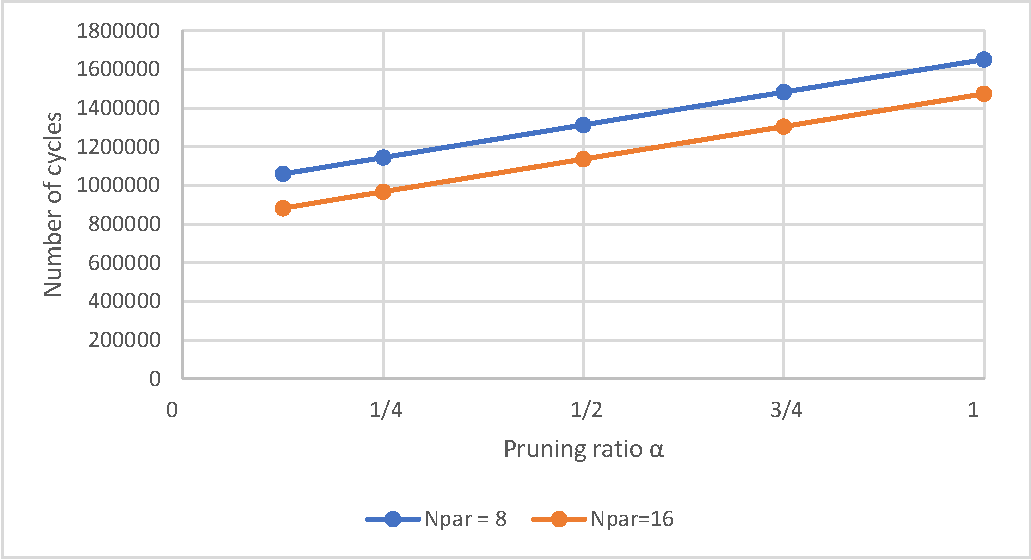
\includegraphics[width=\linewidth]{measur-Nnp.pdf}
            \caption{Number of cycles of the design depending on the pruning ratio for a $N_{par}$ fixed, $N_{par} = 16$ in orange and $N_{par} = 8$ in blue}
            \label{fig:measur-Nnp}
        \end{subfigure}
        %
        \begin{subfigure}[t]{.49\textwidth}
            \centering
            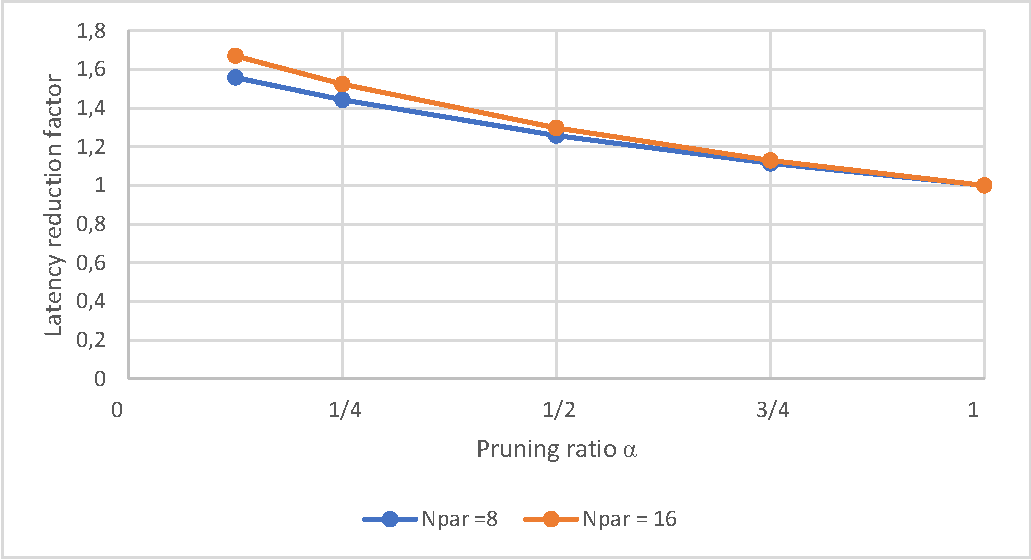
\includegraphics[width=\linewidth]{measur-Nnp-redfac.pdf}
            \caption{Latency reduction factor depending on the pruning ratio for a $N_{par}$ fixed, $N_{par} = 16$ in orange and $N_{par} = 8$ in blue}
            \label{fig:measur-Nnp-redfac}
        \end{subfigure}
        %
        \caption{Number of cycles and Reduction factor of the number of cycles}
    \end{figure}
    %
    \item Second, we conduct similar measurements as above but instead of keeping constant the number of non-pruned weights $N_{np}$, we varied the fetching group size $N_{par}$. The number of cycles depending on the pruning ratio for an $N_{np}$ fixed can be found in Figure \ref{fig:measur-Npar} and the latency reduction factor is shown in Figure \ref{fig:measur-Npar-redfac}. We can observe that as the pruning ratio increases, the latency increases as well (and hence the latency reduction factor decreases). We can also note that we can achieve a bigger latency reduction factor by varying the pruning ratio with $N_{par}$ instead of $N_{np}$.
    For example, in Figure \ref{fig:measur-Nnp-redfac}, the reduction factor corresponding to $\alpha = \frac{1}{8}$ is equal to $1.66$. On the other hand,
    in Figure \ref{fig:measur-Nnp-redfac}, the reduction factor corresponding to $\alpha = \frac{1}{8}$, is equal to $2.79$.
    %
    \begin{figure}[H]
        \centering
        %
        \begin{subfigure}[t]{.49\textwidth}
            \centering
            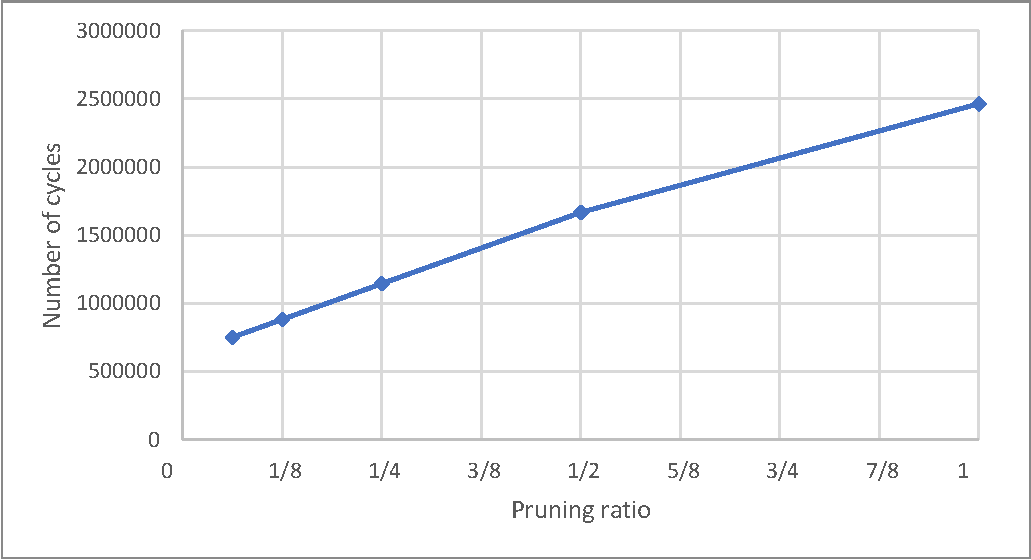
\includegraphics[width=\linewidth]{measur-Npar.pdf}
            \caption{Number of cycles of the design when $N_{np} = 2$}
            \label{fig:measur-Npar}
        \end{subfigure}
        %
        \begin{subfigure}[t]{.49\textwidth}
            \centering
            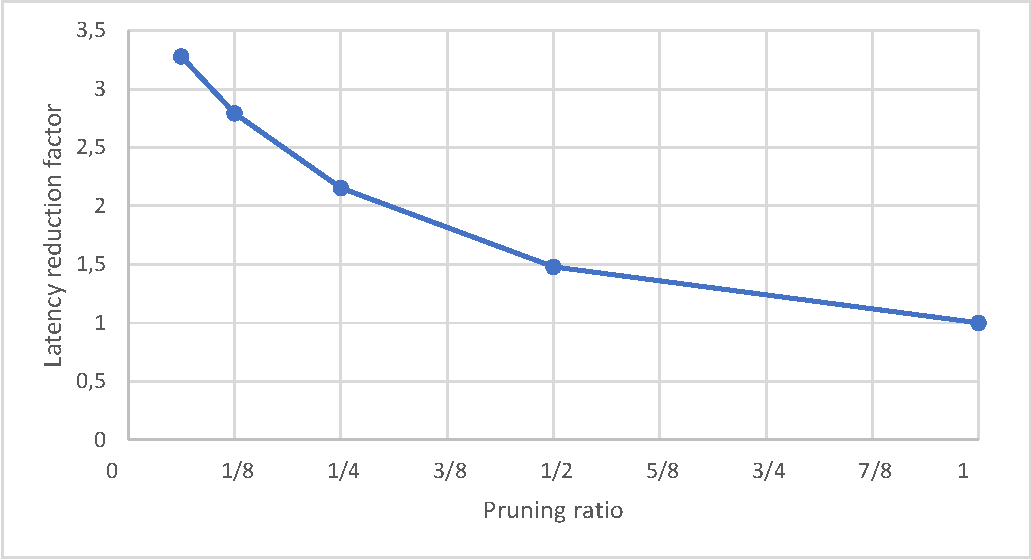
\includegraphics[width=\linewidth]{measur-Npar-redfac.pdf}
            \caption{Latency Reduction factor when $N_{np} = 2$}
            \label{fig:measur-Npar-redfac}
        \end{subfigure}
        %
        \caption{Number of cycles and Reduction factor of the number of cycles for an $N_{p}$ fixed}
    \end{figure}
    %
    %
    \item Finally, we compare the proportion of each component in the overall latency for various pruning parameters. The results can be seen in Figure \ref{fig:ratio-pr}. We observe that if we increase the sparsity, the ratio of cycles spent in the $1 \times 1$ convolution \acrshort{pe} is increased. The latency in the \acrshort{dsc} can therefore be reduced by reducing the pruning ratio. We can also see that the proportion of cycles spent in the \acrshort{dma} is reduced by increasing the fetching group size $N_{par}$.
    \begin{figure}[H]
        \centering
        %
        \begin{subfigure}[t]{.32\textwidth}
            \centering
            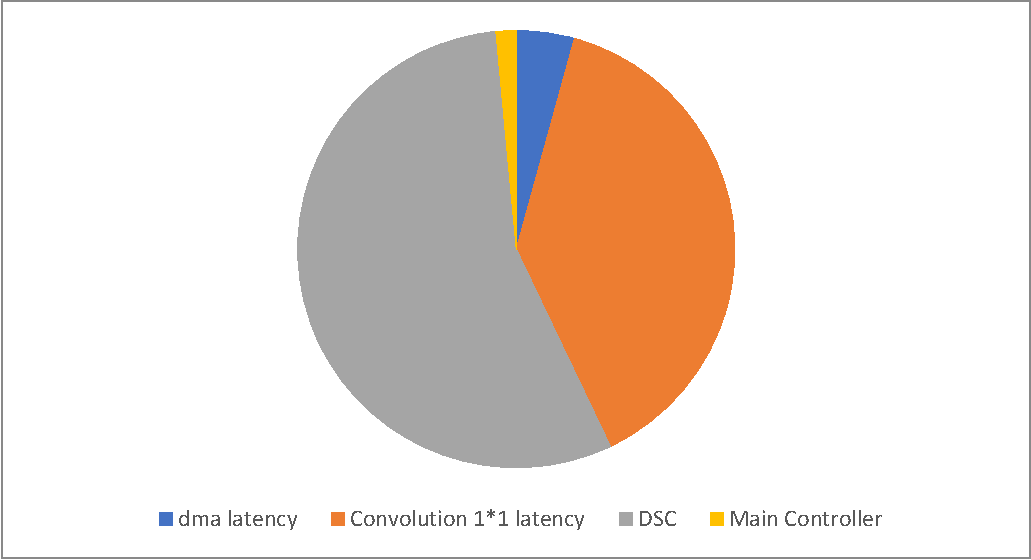
\includegraphics[width=\linewidth]{np8par8prop.pdf}
            \caption{$N_{par} = 8, N_{np} = 8$}
        \end{subfigure}
        %
        \begin{subfigure}[t]{.32\textwidth}
            \centering
            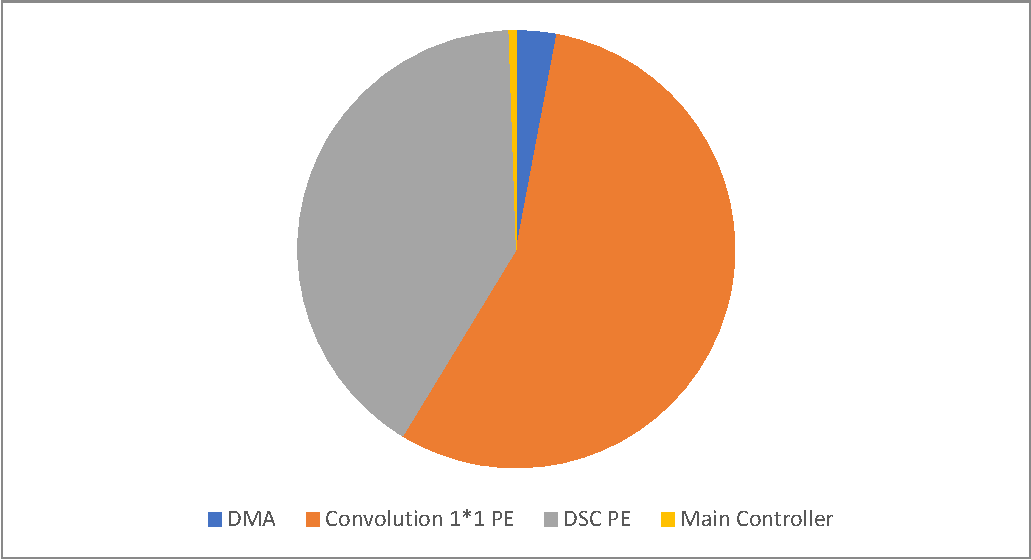
\includegraphics[width=\linewidth]{np2par8prop.pdf}
            \caption{$N_{par} = 8, N_{np} = 2$}
        \end{subfigure}
        %
        \begin{subfigure}[t]{.32\textwidth}
            \centering
            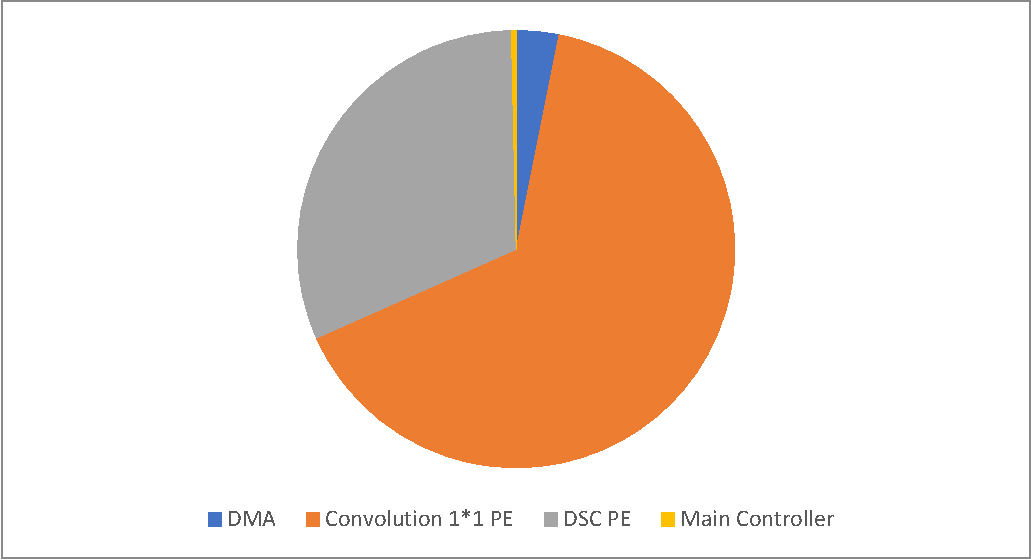
\includegraphics[width=\linewidth]{np2par16prop.pdf}
            \caption{$N_{par} = 16, N_{np} = 2$}
        \end{subfigure}
        %
        \caption{Repartition of the latency across the different components for various pruning parameters}
        \label{fig:ratio-pr}
    \end{figure}
\end{itemize}
%
\subsubsection{Resource usage}
%
Once we have measured the output correctness and the performance of the accelerator, we can measure the resource usage on the target platform. The compilation was performed on Quartus Prime 18.1 Lite Edition. We measured the \acrshort{dsp} utilization, the logic utilization, the number of \acrfull{bram}, and the maximum frequency reachable. The results of the simulations are found in Table \ref{tab:res-simu}.
%
\begin{table}[H]
\begin{tabular}{|l|l|l|l|l|}
\hline
     & DSP & Logic  & BRAM & Frequency [MHz] \\ \hline
    Npar = 4, Nnp = 2 & 45  ( 40 \% ) & 2,006  ( 5 \% ) & 2,104,960  ( 37 \% ) & 114.39 \\ \hline
    Npar = 8, Nnp = 1 & 81 ( 72 \% ) & 2,381  ( 6 \% ) & 2,067,200  ( 37 \% ) & 99.57  \\ \hline
    Npar = 8, Nnp = 2 & 81  ( 72 \% ) & 2,519 ( 6 \% ) & 2,115,840  ( 37 \% ) & 103.36  \\ \hline
    Npar = 8, Nnp = 4 & 83  ( 74 \% ) & 2,678  ( 6 \% ) & 2,213,120 ( 39 \% ) & 85.03  \\ \hline
    Npar = 8, Nnp = 6 & 85  ( 76 \% ) & 2,836  ( 7 \% ) & 2,310,400  ( 41 \% ) & 82.61 \\ \hline
    Npar = 8, Nnp = 8 & 87 ( 78 \% ) & 2,925 ( 7 \% ) & 2,407,680  ( 43 \% ) & 79.85  \\ \hline
    Npar = 16, Nnp = 2 & 112 ( 100 \% ) & 3,484  ( 8 \% ) & 2,132,480 ( 38 \% ) & 97.68  \\ \hline
    Npar = 16, Nnp = 4 & 112  ( 100 \% ) & 3,831  ( 9 \% ) & 2,234,880 ( 39 \% ) & 82.65 \\ \hline
    Npar = 16, Nnp = 8 & 112  ( 100 \% ) & 4,266 ( 10 \% ) & 2,439,680 ( 43 \% ) & 76.31  \\ \hline
    Npar = 16, Nnp = 12 & 112  ( 100 \% ) & 4,789  ( 11 \% ) & 2,644,480  ( 47 \% ) & 66.01 \\ \hline
    Npar = 16, Nnp = 16 & 112 ( 100 \% ) & 5,255  ( 13 \% ) & 2,849,280 ( 50 \% ) & 65.16 \\ \hline
    Npar = 32, Nnp = 2 & 112 ( 100 \% ) & 11,595  ( 28 \% ) & 2,160,640  ( 38 \% ) & 75.79 \\ \hline
\end{tabular}
    \caption{Resource utilization of the network}
    \label{tab:res-simu}
\end{table}

We can deduce, from the results of the compilation results, some relevant information:
\begin{itemize}
    \item The compilation proves the design can be implemented on the target platform.
    \item The increase in $N_{np}$ and $N_{par}$ means bigger on-chip buffers and it is confirmed in the Table.
    \item An increase in the number of $N_{np}$ decreases the operational frequency of the \acrshort{fpga}. This makes sense since an increase in $N_{np}$ means an increase in the number of additions in the convolution. Therefore the critical path becomes larger and the frequency is reduced.
    \item An increase in the number of $N_{par}$ increases also the number of \acrshort{dsp}. This is explained by the depthwise \acrshort{pe} who must perform $N_{par} \times N_{ky} \times N_{kx}$ \acrshort{mac}. According to \textcite{bai_cnn_2018}, the tree adder in Figure \ref{fig:dsc_hardware} is responsible for the limiting frequency. As $N_{par}$ grows, the size of the adder tree increases and the frequency is more limited because the \acrshort{fpga} does not have enough \acrshort{dsp} which are suited for such operation (when $N_{par} = 16$, all \acrshort{dsp} were fully used).
\end{itemize}
%
\subsection{Discussion} \label{subs:discus}
%
In this section, we overview the performance of the accelerator and discuss the obtained results compared to the design objectives.

The ratio of correct outputs indicates that the accelerator provides a logically correct output. Therefore, the implemented design satisfies the fourth design objective: \textquote{\textbf{The proposed architecture provides a logically correct output}}. However, the precision of the output varies according to the pruning parameters, and the accuracy of outputs decreases as $N_{np} \times N_{gr-int}$ increases, which could be a problem if the layer requires a high number of partial sums per output pixel. Still, quantization and integer-arithmetic are known in the literature to suffer from loss of accuracy \cite{wu_quantized_2016, jacob_quantization_2017}. Indeed, \textcite{wu_quantized_2016, jacob_quantization_2017} show that if the training simulates integer arithmetic (and hence the drop of accuracy), the drop of accuracy can be reduced during the training phase.

The performance measurements show that an increase in the sparsity reduces the number of cycles and hence improves the performance of the design. This is explained by two reasons. First, the reduction of $N_{np}$ means that the \acrshort{dsc} \acrshort{pe} has to load fewer weights for each pointwise fetching group. As shown in Figure \ref{fig:c11_hardware}, $N_{np}$ impacts only the number of parallel multiplication and addition in one cycle when performing a $1 \times 1$ convolution. The cycle reduction is not impacted in the $1 \times 1$ convolution \acrshort{pe} because weights and input pixels are loaded in parallel. Second, the increase in the fetching group size $N_{par}$ means that we have fewer fetching groups. We can conclude that $N_{par}$ directly controls the number of convolution and therefore the number of operations. This is why the choice of $N_{par}$ has much impact than $N_{np}$. A bigger $N_{par}$ also means that operation for fetching pixels and weights from the on-chip memory can be more efficiently pipelined, meaning more efficient data accesses. The selection of the highest $N_{par}$ possible should be prioritized over $N_{np}$.

We deduced from the performance measurements that we can improve the latency of the accelerator by applying a smaller pruning ratio and a high $N_{par}$. However, the result of the simulation suggests that the optimal value of $N_{par}$ depends on the resource of the target \acrshort{fpga}. Therefore when implementing the design of the \acrshort{fpga}, the user should find a tradeoff between the pruning parameters, and the constrained resources of the \acrshort{fpga}.
